\chapter{Análise de energia} 

%\label{sec:tp1}

\section{Green Software}
No campo das tecnologias de informação, a poupança de energia costumava ter o seu foco na eficiência energética do hardware, no entanto quando o hardware opera sob software ineficiente, a sua eficiência também pode diminuir substancialmente. Assim, têm sido feitos esforços na medida de otimizar o consumo energético por parte do software, surgindo a definição de \textit{Green Software}, que se descreve como o "software que pode ser desenvolvido e usado eficientemente com o mínimo impacto no ambiente". 

Contudo, esta otimização exige numa primeira instância que se seja capaz de medir e monitorizar o consumo energético, neste contexto surgem ferramentas que permitem  recolher métricas sobre a performance energética. A recolha destas métricas deve ser feita durante o programa em execução e por isso é chamada Análise Dinâmica.   

\subsection{RAPL}
\textit{Running Average Power Limit} foi introduzido pela \textit{Intel} e está presente em todos os processadores Intel x86. O RAPL é uma ferramenta que permite estimar qual a quantidade de energia que está a ser consumida por todos os cores do CPU. 

Assim, no âmbito deste projeto usou-se o RAPL para medir os consumos de energia antes e depois da refabricação do código, de modo a perceber a influência que a eliminação de maus cheiros de código tem sobre a eficiência energética. 

\section{Resultados durante a execução}

Para medir as várias métricas durante a execução do software fornecido foram definidos vários testes independentes, e feitas as medições no programa antes e depois da refabricação. Foi necessário medir várias vezes para garantir o menor erro possível, sendo que os resultados apresentados são a média ponderada das medições. De seguida listam-se os resultados.

\subsection{Tarefa 1}

\textbf{Tarefa:} Operações repetidas, mostrar os dados do cliente 100 vezes.

\begin{figure}[H]
    \centering
    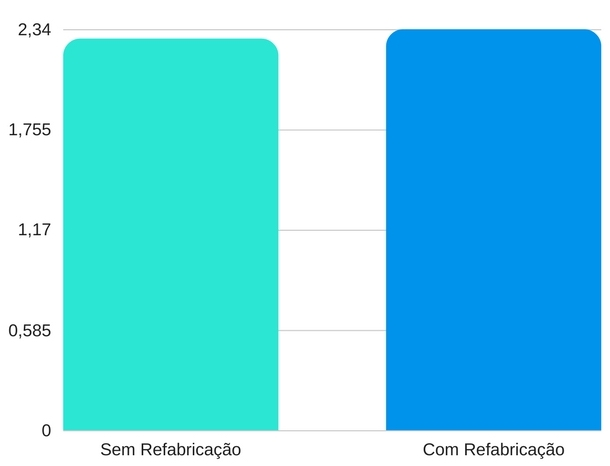
\includegraphics[scale=0.5]{tex/img/graficos/1.jpg}
    \caption{Power Consumption of Dram}
\end{figure}

\begin{figure}[H]
    \centering
    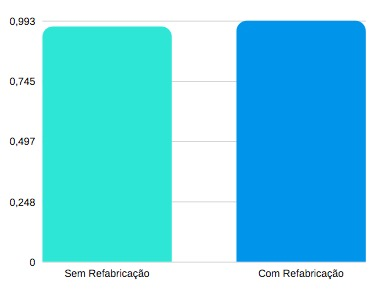
\includegraphics[scale=0.8]{tex/img/graficos/2.jpg}
    \caption{Power Consumption of CPU}
\end{figure}

\begin{figure}[H]
    \centering
    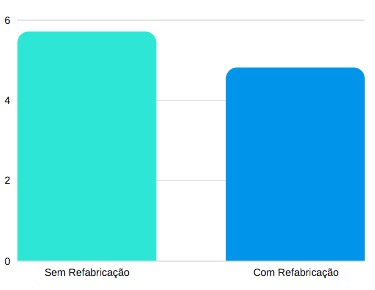
\includegraphics[scale=0.8]{tex/img/graficos/3.jpg}
    \caption{Power Consumption of Package}
\end{figure}


\subsection{Tarefa 2}
\textbf{Tarefa:} Sequência de operações.
\begin{enumerate}
    \setlength{\itemsep}{0pt}
    \setlength{\parskip}{0pt}
    \item Inserir 2 veículos;
    \item Inserir 1 cliente;
    \item Inserir 2 motoristas;
    \item Fazer login motorista1;
    \item Associar motorista1 a veículo 1;
    \item Fazer logout motorista1;
    \item Fazer login motorista2;
    \item Associar motorista2 a veiculo2;
    \item Fazer logout motorista2;
    \item Fazer login cliente;
    \item Chamar veiculo P/ cliente;
    \item Fazer logout cliente;
    \item Logout.
\end{enumerate}

\begin{figure}[H]
    \centering
    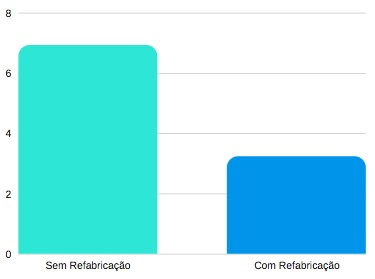
\includegraphics[scale=0.8]{tex/img/graficos/4.jpg}
    \caption{Power Consumption of Dram}
\end{figure}

\begin{figure}[H]
    \centering
    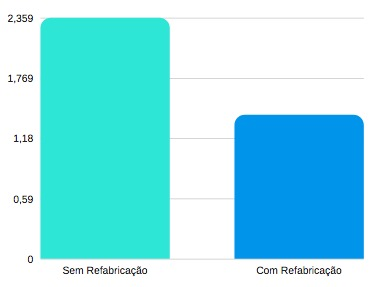
\includegraphics[scale=0.8]{tex/img/graficos/5.jpg}
    \caption{Power Consumption of CPU}
\end{figure}

\begin{figure}[H]
    \centering
    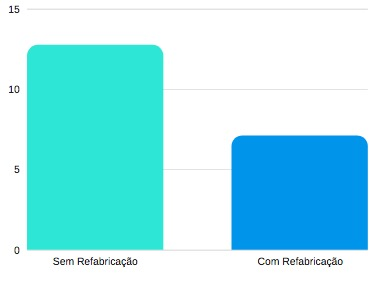
\includegraphics[scale=0.8]{tex/img/graficos/6.jpg}
    \caption{Power Consumption of Package}
\end{figure}

\subsection{Resultados durante os testes unitários}

Para além das medições durante o tempo de execução medimos também a energia usada nos vários testes unitários.
\vspace{5mm}

\textbf{testarAtualizaDados}

\begin{figure}[H]
    \centering
    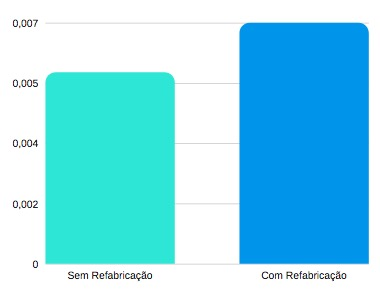
\includegraphics[scale=0.8]{tex/img/graficos/7.jpg}
    \caption{Power Consumption of Dram}
\end{figure}

\begin{figure}[H]
    \centering
    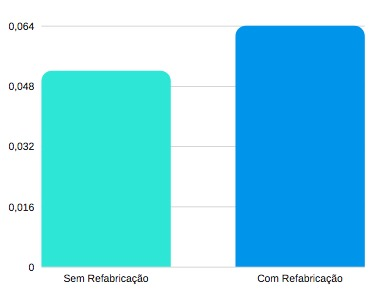
\includegraphics[scale=0.8]{tex/img/graficos/8.jpg}
    \caption{Power Consumption of CPU}
\end{figure}

\begin{figure}[H]
    \centering
    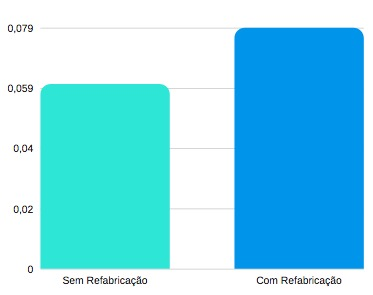
\includegraphics[scale=0.8]{tex/img/graficos/9.jpg}
    \caption{Power Consumption of Package}
\end{figure}

\newpage 
\textbf{testarEquals(atorTeste)}

\begin{figure}[H]
    \centering
    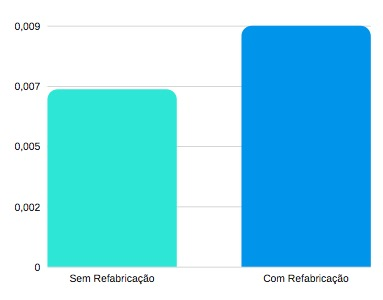
\includegraphics[scale=0.8]{tex/img/graficos/12.jpg}
    \caption{Power Consumption of Dram}
\end{figure}

\begin{figure}[H]
    \centering
    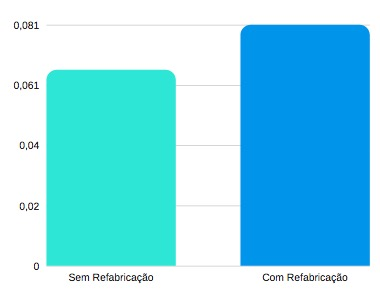
\includegraphics[scale=0.8]{tex/img/graficos/13.jpg}
    \caption{Power Consumption of CPU}
\end{figure}

\begin{figure}[H]
    \centering
    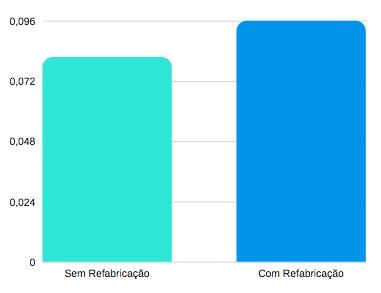
\includegraphics[scale=0.8]{tex/img/graficos/14.jpg}
    \caption{Power Consumption of Package}
\end{figure}


\textbf{testarViagemEntreDatas}

\begin{figure}[H]
    \centering
    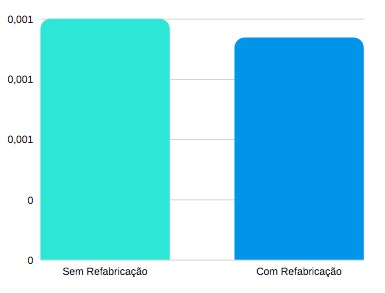
\includegraphics[scale=0.8]{tex/img/graficos/15.jpg}
    \caption{Power Consumption of Dram}
\end{figure}

\begin{figure}[H]
    \centering
    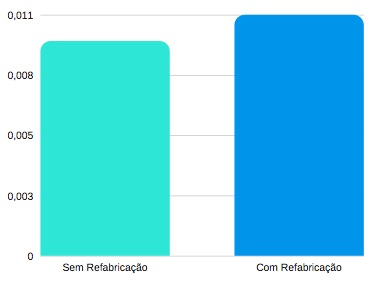
\includegraphics[scale=0.8]{tex/img/graficos/16.jpg}
    \caption{Power Consumption of CPU}
\end{figure}

\begin{figure}[H]
    \centering
    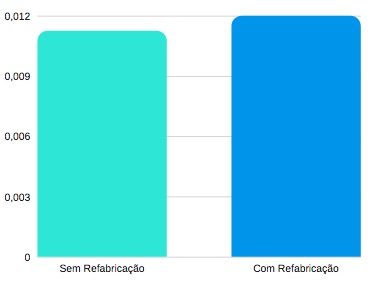
\includegraphics[scale=0.8]{tex/img/graficos/17.jpg}
    \caption{Power Consumption of Package}
\end{figure}

\textbf{testarRegistaViagem}

\begin{figure}[H]
    \centering
    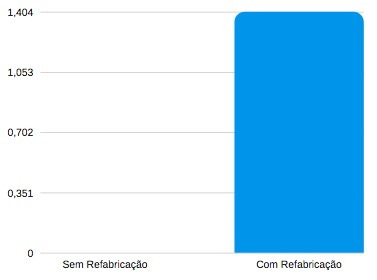
\includegraphics[scale=0.8]{tex/img/graficos/18.jpg}
    \caption{Power Consumption of Dram}
\end{figure}

\begin{figure}[H]
    \centering
    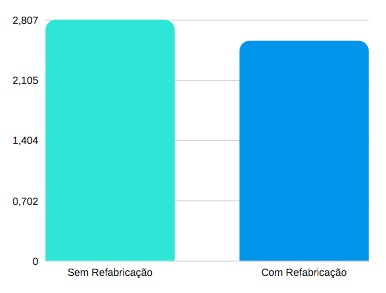
\includegraphics[scale=0.8]{tex/img/graficos/19.jpg}
    \caption{Power Consumption of CPU}
\end{figure}

\begin{figure}[H]
    \centering
    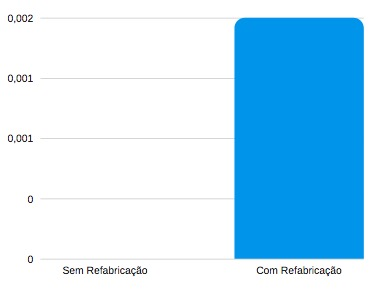
\includegraphics[scale=0.8]{tex/img/graficos/20.jpg}
    \caption{Power Consumption of Package}
\end{figure}

\textbf{testarMaiorDesvio}

\begin{figure}[H]
    \centering
    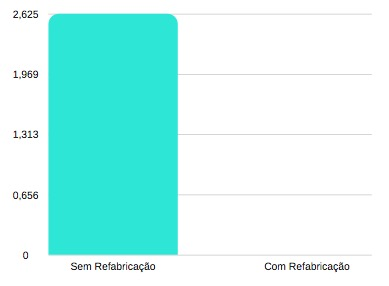
\includegraphics[scale=0.8]{tex/img/graficos/21.jpg}
    \caption{Power Consumption of Dram}
\end{figure}

\begin{figure}[H]
    \centering
    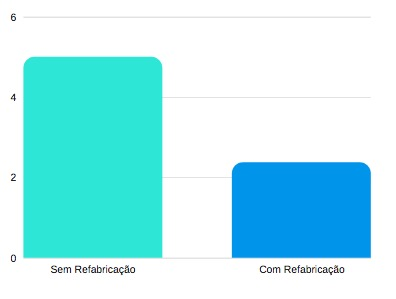
\includegraphics[scale=0.8]{tex/img/graficos/22.jpg}
    \caption{Power Consumption of CPU}
\end{figure}

\begin{figure}[H]
    \centering
    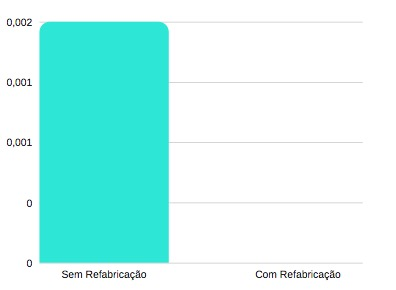
\includegraphics[scale=0.8]{tex/img/graficos/23.jpg}
    \caption{Power Consumption of Package}
\end{figure}

\textbf{testarEquals(coordenadaTest)}

\begin{figure}[H]
    \centering
    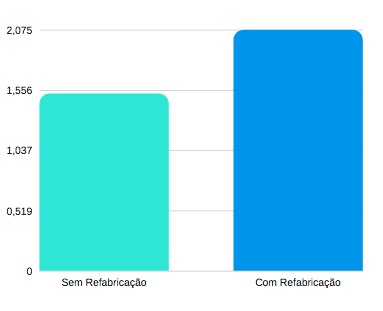
\includegraphics[scale=0.8]{tex/img/graficos/24.jpg}
    \caption{Power Consumption of Dram}
\end{figure}

\begin{figure}[H]
    \centering
    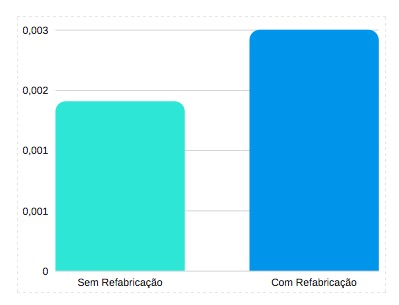
\includegraphics[scale=0.8]{tex/img/graficos/25.jpg}
    \caption{Power Consumption of CPU}
\end{figure}

\begin{figure}[H]
    \centering
    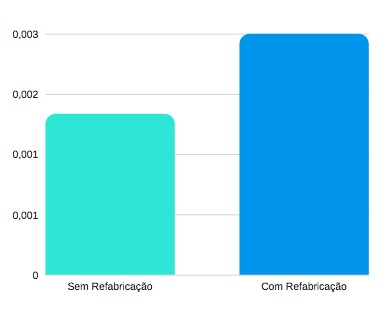
\includegraphics[scale=0.8]{tex/img/graficos/26.jpg}
    \caption{Power Consumption of Package}
\end{figure}

\textbf{testarDistancia}

\begin{figure}[H]
    \centering
    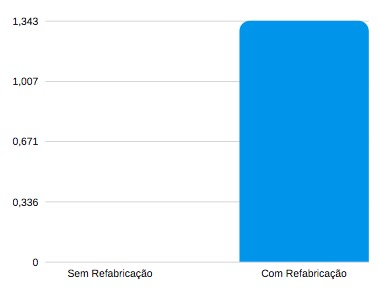
\includegraphics[scale=0.8]{tex/img/graficos/27.jpg}
    \caption{Power Consumption of Dram}
\end{figure}

\begin{figure}[H]
    \centering
    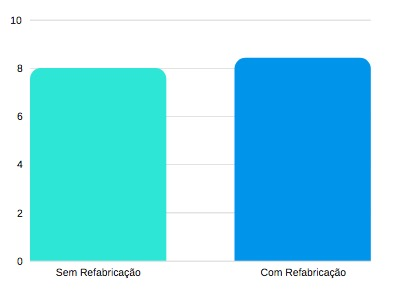
\includegraphics[scale=0.8]{tex/img/graficos/28.jpg}
    \caption{Power Consumption of CPU}
\end{figure}

\begin{figure}[H]
    \centering
    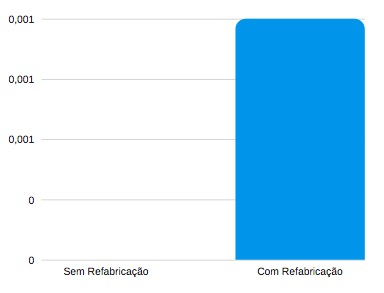
\includegraphics[scale=0.8]{tex/img/graficos/29.jpg}
    \caption{Power Consumption of Package}
\end{figure}


